\documentclass[dvipsnames]{article}
\usepackage{tikz,pgfplots}
\usepackage{tikz-qtree}
\usepackage{units}
\usepackage{braket}
\usepackage[]{xcolor}
\pgfplotsset{compat=1.8}
%\pgfplotsset{colormap={mix}{
%	color(0cm)=(blue);
%	color(1cm)=(green);
%	color(2cm)=(yellow)
%	color(3cm)=(red)}}

\usetikzlibrary{patterns,shadows,fadings,positioning,trees,calc}
\usepgfplotslibrary{external}
\tikzexternalize


\tikzfading[name=fade inside,
         inner color=transparent!80,
         outer color=transparent!30]
\tikzfading[name=fade out,
         inner color=transparent!0,
         outer color=transparent!90]


%\definecolor{diplom1}{rgb}{0.0 0.4 1.0}
%\definecolor{diplom2}{rgb}{0.0 0.0 0.6}
\definecolor{diplom1}{RGB}{101 156 239}
\definecolor{diplom2}{RGB}{000 000 128}
\definecolor{diplom3}{RGB}{153,0,0} %unirot
\definecolor{diplom4}{RGB}{232,215,23}
\definecolor{diplom5}{RGB}{51,37,60}

\definecolor{unirot}{RGB}{153,0,0}
\definecolor{unirot_hell}{RGB}{255,228,225}
\definecolor{lightblue}{RGB}{242.2,249.88,255}

\pgfplotsset{colormap={diplom1s}{
       color(0cm)=(white);
       color(1cm)=(diplom1);
       color(10cm)=(diplom1)}}
\pgfplotsset{colormap={diplom2s}{
       color(0cm)=(white);
       color(1cm)=(diplom1);
       color(2cm)=(diplom2)}}
\pgfplotsset{colormap={blues}{
       color(0cm)=(diplom2);
       color(1cm)=(diplom1);
       color(2cm)=(white);
       color(3cm)=(diplom1);
       color(4cm)=(diplom2)}}

\pgfplotsset{
   /pgfplots/bar  cycle  list/.style={/pgfplots/cycle  list={%
        {diplom1,  fill=diplom1!30!white,  mark=none,very thick},%
        {diplom2,  fill=diplom2!30!white,  mark=none,very thick},%
        {diplom3,  fill=diplom3!30!white,  mark=none,very thick},%
        {orange,   fill=orange!30!white,   mark=none,very thick},%
        {LimeGreen,fill=LimeGreen!30!white,mark=none,very thick},%
        {Fuchsia,  fill=Fuchsia!30!white,  mark=none,very thick},%
        {Green,    fill=Green!30!white,    mark=none,very thick},%
        {Goldenrod,fill=Goldenrod!30!white,mark=none,very thick},%
     }
   },
}

\pgfplotsset{
  cycle  list={%
        {diplom1,  mark=none,very thick},%
        {diplom2,  mark=none,very thick},%
        {diplom3,  mark=none,very thick},%
        {orange,   mark=none,very thick},%
        {LimeGreen,mark=none,very thick},%
        {Fuchsia,  mark=none,very thick},%
        {Green,    mark=none,very thick},%
        {Goldenrod,mark=none,very thick},%
     }
   }


\begin{document}

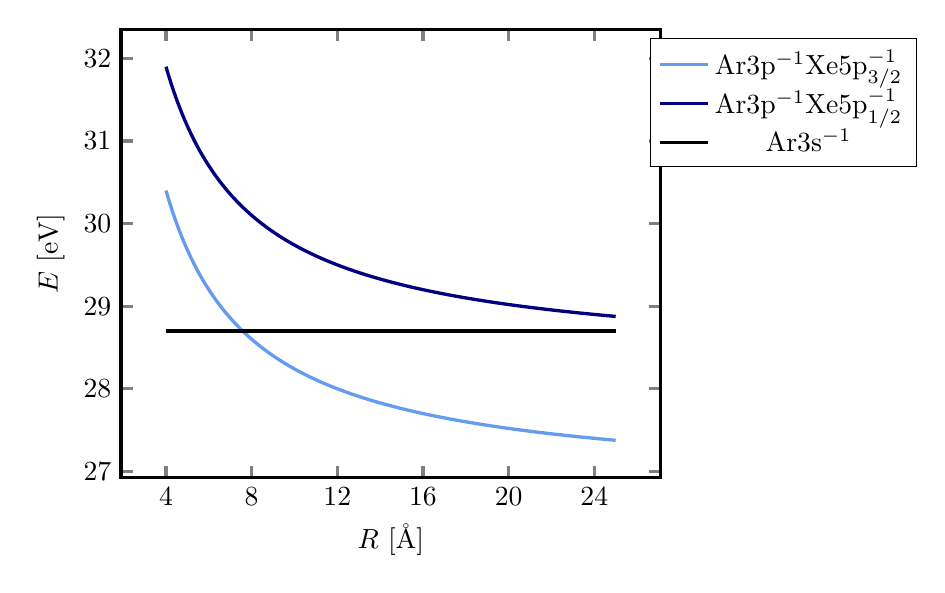
\begin{tikzpicture}
    \begin{axis}[domain=4.0:25,
                 samples = 200,
                 xtick={4.0,8.0,...,24},
                 %xticklabels={$-\pi$,$-\frac \pi 2$,0,$\frac \pi 2$,$\pi$},
                 %cycle list name = exotic,
                 legend style={anchor= north west},
                 xlabel={$R$ [\AA]},
                 ylabel={$E$ [eV]},
                 axis line style = very thick,
                 tick style = very thick,
                 ]

      \addplot+[
                mark = none,
               ]
               {15.3 + 11.5 + 14.39964 / x};
      \addlegendentry{Ar3p$^{-1}$Xe5p$_{3/2}^{-1}$};

      \addplot+[
                mark = none,
               ]
               {15.3 + 13.0 + 14.39964 / x};
      \addlegendentry{Ar3p$^{-1}$Xe5p$_{1/2}^{-1}$};


      \addplot+[
                mark = none,
                black,
               ]
               {28.7};
      \addlegendentry{Ar3s$^{-1}$};
      %\draw[] (axis cs:\pgfkeysvalueof{/pgfplots/xmin},29.239) -- (axis cs:\pgfkeysvalueof{/pgfplots/xmax},29.239);
    \end{axis}
\end{tikzpicture}


%\begin{tikzpicture}[scale=1.0]

\begin{axis}[%scale=1.5,
             domain=0:6,
             restrict expr to domain={x}{0:6},
             %restrict expr to domain={y}{1.0E-12:7},
             xlabel={E [eV]},
             %xtick={30,50,...,170},
             %xticklabels={2,4,6,8,10,12,15,20,25},
             %ytick={-1.0,-0.8,...,1.0},
             %yticklabels={1.0,0.8,0.6,0.4,0.2,0.0,0.2,0.4,0.6,0.8,1.0},
             ylabel={$\Gamma$ [eV]},
             scale only axis,
             width=\textwidth-1.5cm,
             height=8cm,
             %ybar stacked
             ]


%%%%%%%%%%%%%%%%%%%%%%%%%%%%%%%%%%%%%%%%%%%%%%%%%%%%%%%%%%%%%%%%%%%%%%%%%%%%%%%%%%%%%%

\addplot+[ycomb,
         mark=.,
         very thick,
         diplom1,
         forget plot
        ]
        table[
        x expr = \thisrowno{0},
        y expr = \thisrowno{1}
        ]
        {../data/Ar13Xe25-ICD};
        \addlegendimage{line legend, diplom1, very thick};
        \addlegendentry{Ar$_{13}$Xe$_{25}$ -- ICD};

\addplot[
         mark=none,
         diplom1,
         very thick,
         %dotted
         forget plot
         ]
         table[
         x expr=\thisrowno{0},
         y expr=\thisrowno{1}
         ]
        {../data/Ar13Xe25-ICD.sp};
         %\addlegendentry{ICD spectrum};
%%%%%%%%%%%%%%%%%%%%%%%%%%%%%%%%%%%%%%%%%%%%%%%%%%%%%%%%%%%%%%%%%%%%%%%%%%%%%%%%%%%%%%

\addplot+[ycomb,
         mark=.,
         very thick,
         diplom2,
         forget plot
        ]
        table[
        x expr = \thisrowno{0},
        y expr = \thisrowno{1}
        ]
        {../data/Ar13Xe25-ETMD};
        \addlegendimage{line legend, diplom2, very thick};
        \addlegendentry{Ar$_{13}$Xe$_{25}$ -- ETMD};

\addplot[
         mark=none,
         diplom2,
         very thick,
         %dotted
         ]
         table[
         x expr=\thisrowno{0},
         y expr=\thisrowno{1}
         ]
        {../data/Ar13Xe25-ETMD.sp};
         %\addlegendentry{ETMD spectrum};
%%%%%%%%%%%%%%%%%%%%%%%%%%%%%%%%%%%%%%%%%%%%%%%%%%%%%%%%%%%%%%%%%%%%%%%%%%%%%%%%%%%%%%




\end{axis}
\end{tikzpicture}
\\
%\begin{tikzpicture}[scale=1.0]

\begin{axis}[%scale=1.5,
             domain=0:6,
             restrict expr to domain={x}{0:6},
             %restrict expr to domain={y}{1.0E-12:7},
             xlabel={E [eV]},
             %xtick={30,50,...,170},
             %xticklabels={2,4,6,8,10,12,15,20,24},
             %ytick={-1.0,-0.8,...,1.0},
             %yticklabels={1.0,0.8,0.6,0.4,0.2,0.0,0.2,0.4,0.6,0.8,1.0},
             ylabel={$\Gamma$ [eV]},
             scale only axis,
             width=\textwidth-1.5cm,
             height=8cm,
             %ybar stacked
             ]


%%%%%%%%%%%%%%%%%%%%%%%%%%%%%%%%%%%%%%%%%%%%%%%%%%%%%%%%%%%%%%%%%%%%%%%%%%%%%%%%%%%%%%

\addplot+[ycomb,
         mark=.,
         very thick,
         diplom1,
         forget plot
        ]
        table[
        x expr = \thisrowno{0},
        y expr = \thisrowno{1}
        ]
        {../data/Ar14Xe24-ICD};
        \addlegendimage{line legend, diplom1, very thick};
        \addlegendentry{Ar$_{14}$Xe$_{24}$ -- ICD};

\addplot[
         mark=none,
         diplom1,
         very thick,
         %dotted
         forget plot
         ]
         table[
         x expr=\thisrowno{0},
         y expr=\thisrowno{1}
         ]
        {../data/Ar14Xe24-ICD.sp};
         %\addlegendentry{ICD spectrum};
%%%%%%%%%%%%%%%%%%%%%%%%%%%%%%%%%%%%%%%%%%%%%%%%%%%%%%%%%%%%%%%%%%%%%%%%%%%%%%%%%%%%%%

\addplot+[ycomb,
         mark=.,
         very thick,
         diplom2,
         forget plot
        ]
        table[
        x expr = \thisrowno{0},
        y expr = \thisrowno{1}
        ]
        {../data/Ar14Xe24-ETMD};
        \addlegendimage{line legend, diplom2, very thick};
        \addlegendentry{Ar$_{14}$Xe$_{24}$ -- ETMD};

\addplot[
         mark=none,
         diplom2,
         very thick,
         %dotted
         ]
         table[
         x expr=\thisrowno{0},
         y expr=\thisrowno{1}
         ]
        {../data/Ar14Xe24-ETMD.sp};
         %\addlegendentry{ETMD spectrum};
%%%%%%%%%%%%%%%%%%%%%%%%%%%%%%%%%%%%%%%%%%%%%%%%%%%%%%%%%%%%%%%%%%%%%%%%%%%%%%%%%%%%%%




\end{axis}
\end{tikzpicture}
\\
%\begin{tikzpicture}[scale=1.0]

\begin{axis}[%scale=1.5,
             domain=0:6,
             restrict expr to domain={x}{0:6},
             %restrict expr to domain={y}{1.0E-12:7},
             xlabel={E [eV]},
             %xtick={30,50,...,170},
             %xticklabels={2,4,6,8,10,12,15,20,25},
             %ytick={-1.0,-0.8,...,1.0},
             %yticklabels={1.0,0.8,0.6,0.4,0.2,0.0,0.2,0.4,0.6,0.8,1.0},
             ylabel={$\Gamma$ [eV]},
             scale only axis,
             width=\textwidth-1.5cm,
             height=8cm,
             %ybar stacked
             ]


%%%%%%%%%%%%%%%%%%%%%%%%%%%%%%%%%%%%%%%%%%%%%%%%%%%%%%%%%%%%%%%%%%%%%%%%%%%%%%%%%%%%%%

\addplot+[ycomb,
         mark=.,
         very thick,
         diplom1,
         forget plot
        ]
        table[
        x expr = \thisrowno{0},
        y expr = \thisrowno{1}
        ]
        {../data/Ar25Xe13-ICD};
        \addlegendimage{line legend, diplom1, very thick};
        \addlegendentry{Ar$_{25}$Xe$_{13}$ -- ICD};

\addplot[
         mark=none,
         diplom1,
         very thick,
         %dotted
         forget plot
         ]
         table[
         x expr=\thisrowno{0},
         y expr=\thisrowno{1}
         ]
        {../data/Ar25Xe13-ICD.sp};
         %\addlegendentry{ICD spectrum};
%%%%%%%%%%%%%%%%%%%%%%%%%%%%%%%%%%%%%%%%%%%%%%%%%%%%%%%%%%%%%%%%%%%%%%%%%%%%%%%%%%%%%%

\addplot+[ycomb,
         mark=.,
         very thick,
         diplom2,
         forget plot
        ]
        table[
        x expr = \thisrowno{0},
        y expr = \thisrowno{1}
        ]
        {../data/Ar25Xe13-ETMD};
        \addlegendimage{line legend, diplom2, very thick};
        \addlegendentry{Ar$_{25}$Xe$_{13}$ -- ETMD};

\addplot[
         mark=none,
         diplom2,
         very thick,
         %dotted
         ]
         table[
         x expr=\thisrowno{0},
         y expr=\thisrowno{1}
         ]
        {../data/Ar25Xe13-ETMD.sp};
         %\addlegendentry{ETMD spectrum};
%%%%%%%%%%%%%%%%%%%%%%%%%%%%%%%%%%%%%%%%%%%%%%%%%%%%%%%%%%%%%%%%%%%%%%%%%%%%%%%%%%%%%%




\end{axis}
\end{tikzpicture}
\\
%\begin{tikzpicture}[scale=1.0]

\begin{axis}[%scale=1.5,
             domain=0:6,
             restrict expr to domain={x}{0:6},
             %restrict expr to domain={y}{1.0E-12:7},
             xlabel={E [eV]},
             %xtick={30,50,...,170},
             %xticklabels={2,4,6,8,10,12,15,20,5},
             %ytick={-1.0,-0.8,...,1.0},
             %yticklabels={1.0,0.8,0.6,0.4,0.2,0.0,0.2,0.4,0.6,0.8,1.0},
             ylabel={$\Gamma$ [eV]},
             scale only axis,
             width=\textwidth-1.5cm,
             height=8cm,
             %ybar stacked
             ]


%%%%%%%%%%%%%%%%%%%%%%%%%%%%%%%%%%%%%%%%%%%%%%%%%%%%%%%%%%%%%%%%%%%%%%%%%%%%%%%%%%%%%%

\addplot+[ycomb,
         mark=.,
         very thick,
         diplom1,
         forget plot
        ]
        table[
        x expr = \thisrowno{0},
        y expr = \thisrowno{1}
        ]
        {../data/Ar33Xe5-ICD};
        \addlegendimage{line legend, diplom1, very thick};
        \addlegendentry{Ar$_{33}$Xe$_{5}$ -- ICD};

\addplot[
         mark=none,
         diplom1,
         very thick,
         %dotted
         forget plot
         ]
         table[
         x expr=\thisrowno{0},
         y expr=\thisrowno{1}
         ]
        {../data/Ar33Xe5-ICD.sp};
         %\addlegendentry{ICD spectrum};
%%%%%%%%%%%%%%%%%%%%%%%%%%%%%%%%%%%%%%%%%%%%%%%%%%%%%%%%%%%%%%%%%%%%%%%%%%%%%%%%%%%%%%

\addplot+[ycomb,
         mark=.,
         very thick,
         diplom2,
         forget plot
        ]
        table[
        x expr = \thisrowno{0},
        y expr = \thisrowno{1}
        ]
        {../data/Ar33Xe5-ETMD};
        \addlegendimage{line legend, diplom2, very thick};
        \addlegendentry{Ar$_{33}$Xe$_{5}$ -- ETMD};

\addplot[
         mark=none,
         diplom2,
         very thick,
         %dotted
         ]
         table[
         x expr=\thisrowno{0},
         y expr=\thisrowno{1}
         ]
        {../data/Ar33Xe5-ETMD.sp};
         %\addlegendentry{ETMD spectrum};
%%%%%%%%%%%%%%%%%%%%%%%%%%%%%%%%%%%%%%%%%%%%%%%%%%%%%%%%%%%%%%%%%%%%%%%%%%%%%%%%%%%%%%




\end{axis}
\end{tikzpicture}
 \\
%\begin{tikzpicture}[scale=1.0]

\begin{axis}[%scale=1.5,
             domain=0:6,
             restrict expr to domain={x}{0:6},
             %restrict expr to domain={y}{1.0E-12:7},
             xlabel={E [eV]},
             %xtick={30,50,...,170},
             %xticklabels={2,4,6,8,10,12,15,20,4},
             %ytick={-1.0,-0.8,...,1.0},
             %yticklabels={1.0,0.8,0.6,0.4,0.2,0.0,0.2,0.4,0.6,0.8,1.0},
             ylabel={$\Gamma$ [eV]},
             scale only axis,
             width=\textwidth-1.5cm,
             height=8cm,
             %ybar stacked
             ]


%%%%%%%%%%%%%%%%%%%%%%%%%%%%%%%%%%%%%%%%%%%%%%%%%%%%%%%%%%%%%%%%%%%%%%%%%%%%%%%%%%%%%%

\addplot+[ycomb,
         mark=.,
         very thick,
         diplom1,
         forget plot
        ]
        table[
        x expr = \thisrowno{0},
        y expr = \thisrowno{1}
        ]
        {../data/Ar34Xe4-ICD};
        \addlegendimage{line legend, diplom1, very thick};
        \addlegendentry{Ar$_{34}$Xe$_{4}$ -- ICD};

\addplot[
         mark=none,
         diplom1,
         very thick,
         %dotted
         forget plot
         ]
         table[
         x expr=\thisrowno{0},
         y expr=\thisrowno{1}
         ]
        {../data/Ar34Xe4-ICD.sp};
         %\addlegendentry{ICD spectrum};
%%%%%%%%%%%%%%%%%%%%%%%%%%%%%%%%%%%%%%%%%%%%%%%%%%%%%%%%%%%%%%%%%%%%%%%%%%%%%%%%%%%%%%

\addplot+[ycomb,
         mark=.,
         very thick,
         diplom2,
         forget plot
        ]
        table[
        x expr = \thisrowno{0},
        y expr = \thisrowno{1}
        ]
        {../data/Ar34Xe4-ETMD};
        \addlegendimage{line legend, diplom2, very thick};
        \addlegendentry{Ar$_{34}$Xe$_{4}$ -- ETMD};

\addplot[
         mark=none,
         diplom2,
         very thick,
         %dotted
         ]
         table[
         x expr=\thisrowno{0},
         y expr=\thisrowno{1}
         ]
        {../data/Ar34Xe4-ETMD.sp};
         %\addlegendentry{ETMD spectrum};
%%%%%%%%%%%%%%%%%%%%%%%%%%%%%%%%%%%%%%%%%%%%%%%%%%%%%%%%%%%%%%%%%%%%%%%%%%%%%%%%%%%%%%




\end{axis}
\end{tikzpicture}
 \\
%\begin{tikzpicture}[scale=1.0]

\begin{axis}[%scale=1.5,
             domain=0:6,
             restrict expr to domain={x}{0:6},
             %restrict expr to domain={y}{1.0E-12:7},
             xlabel={E [eV]},
             %xtick={30,50,...,170},
             %xticklabels={2,4,6,8,10,12,15,20,2},
             %ytick={-1.0,-0.8,...,1.0},
             %yticklabels={1.0,0.8,0.6,0.4,0.2,0.0,0.2,0.4,0.6,0.8,1.0},
             ylabel={$\Gamma$ [eV]},
             scale only axis,
             width=\textwidth-1.5cm,
             height=8cm,
             %ybar stacked
             ]


%%%%%%%%%%%%%%%%%%%%%%%%%%%%%%%%%%%%%%%%%%%%%%%%%%%%%%%%%%%%%%%%%%%%%%%%%%%%%%%%%%%%%%

\addplot+[ycomb,
         mark=.,
         very thick,
         diplom1,
         forget plot
        ]
        table[
        x expr = \thisrowno{0},
        y expr = \thisrowno{1}
        ]
        {../data/Ar36Xe2-ICD};
        \addlegendimage{line legend, diplom1, very thick};
        \addlegendentry{Ar$_{36}$Xe$_{2}$ -- ICD};

\addplot[
         mark=none,
         diplom1,
         very thick,
         %dotted
         forget plot
         ]
         table[
         x expr=\thisrowno{0},
         y expr=\thisrowno{1}
         ]
        {../data/Ar36Xe2-ICD.sp};
         %\addlegendentry{ICD spectrum};
%%%%%%%%%%%%%%%%%%%%%%%%%%%%%%%%%%%%%%%%%%%%%%%%%%%%%%%%%%%%%%%%%%%%%%%%%%%%%%%%%%%%%%

\addplot+[ycomb,
         mark=.,
         very thick,
         diplom2,
         forget plot
        ]
        table[
        x expr = \thisrowno{0},
        y expr = \thisrowno{1}
        ]
        {../data/Ar36Xe2-ETMD};
        \addlegendimage{line legend, diplom2, very thick};
        \addlegendentry{Ar$_{36}$Xe$_{2}$ -- ETMD};

\addplot[
         mark=none,
         diplom2,
         very thick,
         %dotted
         ]
         table[
         x expr=\thisrowno{0},
         y expr=\thisrowno{1}
         ]
        {../data/Ar36Xe2-ETMD.sp};
         %\addlegendentry{ETMD spectrum};
%%%%%%%%%%%%%%%%%%%%%%%%%%%%%%%%%%%%%%%%%%%%%%%%%%%%%%%%%%%%%%%%%%%%%%%%%%%%%%%%%%%%%%




\end{axis}
\end{tikzpicture}
 \\
%\begin{tikzpicture}[scale=1.0]

\begin{axis}[%scale=1.5,
             domain=0:6,
             restrict expr to domain={x}{0:6},
             %restrict expr to domain={y}{1.0E-12:7},
             xlabel={E [eV]},
             %xtick={30,50,...,170},
             %xticklabels={2,4,6,8,10,12,15,20,35},
             %ytick={-1.0,-0.8,...,1.0},
             %yticklabels={1.0,0.8,0.6,0.4,0.2,0.0,0.2,0.4,0.6,0.8,1.0},
             ylabel={$\Gamma$ [eV]},
             scale only axis,
             width=\textwidth-1.5cm,
             height=8cm,
             %ybar stacked
             ]


%%%%%%%%%%%%%%%%%%%%%%%%%%%%%%%%%%%%%%%%%%%%%%%%%%%%%%%%%%%%%%%%%%%%%%%%%%%%%%%%%%%%%%

\addplot+[ycomb,
         mark=.,
         very thick,
         diplom1,
         forget plot
        ]
        table[
        x expr = \thisrowno{0},
        y expr = \thisrowno{1}
        ]
        {../data/Ar3Xe35-ICD};
        \addlegendimage{line legend, diplom1, very thick};
        \addlegendentry{Ar$_{3}$Xe$_{35}$ -- ICD};

\addplot[
         mark=none,
         diplom1,
         very thick,
         %dotted
         forget plot
         ]
         table[
         x expr=\thisrowno{0},
         y expr=\thisrowno{1}
         ]
        {../data/Ar3Xe35-ICD.sp};
         %\addlegendentry{ICD spectrum};
%%%%%%%%%%%%%%%%%%%%%%%%%%%%%%%%%%%%%%%%%%%%%%%%%%%%%%%%%%%%%%%%%%%%%%%%%%%%%%%%%%%%%%

\addplot+[ycomb,
         mark=.,
         very thick,
         diplom2,
         forget plot
        ]
        table[
        x expr = \thisrowno{0},
        y expr = \thisrowno{1}
        ]
        {../data/Ar3Xe35-ETMD};
        \addlegendimage{line legend, diplom2, very thick};
        \addlegendentry{Ar$_{3}$Xe$_{35}$ -- ETMD};

\addplot[
         mark=none,
         diplom2,
         very thick,
         %dotted
         ]
         table[
         x expr=\thisrowno{0},
         y expr=\thisrowno{1}
         ]
        {../data/Ar3Xe35-ETMD.sp};
         %\addlegendentry{ETMD spectrum};
%%%%%%%%%%%%%%%%%%%%%%%%%%%%%%%%%%%%%%%%%%%%%%%%%%%%%%%%%%%%%%%%%%%%%%%%%%%%%%%%%%%%%%




\end{axis}
\end{tikzpicture}
 \\

%\begin{tikzpicture}[scale=1.0]

\begin{axis}[%scale=1.5,
             domain=0:6,
             restrict expr to domain={x}{0:6},
             %restrict expr to domain={y}{1.0E-12:7},
             xlabel={E [eV]},
             %xtick={30,50,...,170},
             %xticklabels={2,4,6,8,10,12,15,20,25},
             %ytick={-1.0,-0.8,...,1.0},
             %yticklabels={1.0,0.8,0.6,0.4,0.2,0.0,0.2,0.4,0.6,0.8,1.0},
             ylabel={$\Gamma$ [eV]},
             scale only axis,
             width=\textwidth-1.5cm,
             height=8cm,
             %ybar stacked
             ]

%ICD

\addplot+[ycomb,
         mark=.,
         very thick,
         diplom1,
         forget plot
        ]
        table[
        x expr = \thisrowno{0},
        y expr = \thisrowno{1}
        ]
        {../data/2_2endtop_ICD.dat_intadd};
        \addlegendimage{line legend, diplom1, very thick};
        \addlegendentry{furthest -- ICD};

\addplot[
         mark=none,
         diplom1,
         very thick,
         forget plot
         %dashed
         ]
         table[
         x expr=\thisrowno{0},
         y expr=\thisrowno{1}
         ]
        {../data/2_2endtop_ICD.dat_intadd.inp.sp};
%%%%%%%%%%%%%%%%%%%%%%%%%%%%%%%%%%%%%%%%%%%%%%%%%%%

\addplot+[ycomb,
         mark=.,
         very thick,
         diplom2,
         forget plot
        ]
        table[
        x expr = \thisrowno{0},
        y expr = \thisrowno{1}
        ]
        {../data/2_2endtop_ETMD.dat_intadd};
        \addlegendimage{line legend, diplom2, very thick};
         \addlegendentry{furthest -- ETMD};

\addplot[
         mark=none,
         diplom2,
         very thick,
         forget plot
         %dashed
         ]
         table[
         x expr=\thisrowno{0},
         y expr=\thisrowno{1}
         ]
        {../data/2_2endtop_ETMD.dat_intadd.inp.sp};
%%%%%%%%%%%%%%%%%%%%%%%%%%%%%%%%%%%%%%%%%%%%%%%%%%%


\addplot+[ycomb,
         mark=.,
         very thick,
         Green,
         forget plot
        ]
        table[
        x expr = \thisrowno{0},
        y expr = \thisrowno{1}
        ]
        {../data/xear_2_2_midtop_ICD.dat_intadd};
        \addlegendimage{line legend, Green, very thick};
        \addlegendentry{middle -- ICD};

\addplot[
         mark=none,
         Green,
         very thick,
         forget plot
         %dashed
         ]
         table[
         x expr=\thisrowno{0},
         y expr=\thisrowno{1}
         ]
        {../data/xear_2_2_midtop_ICD.dat_intadd.inp.sp};
%%%%%%%%%%%%%%%%%%%%%%%%%%%%%%%%%%%%%%%%%%%%%%%%%%%

\addplot+[ycomb,
         mark=.,
         very thick,
         LimeGreen,
         forget plot
        ]
        table[
        x expr = \thisrowno{0},
        y expr = \thisrowno{1}
        ]
        {../data/xear_2_2_midtop_ETMD.dat_intadd};
        \addlegendimage{line legend, LimeGreen, very thick};
         \addlegendentry{middle -- ETMD};

\addplot[
         mark=none,
         LimeGreen,
         very thick,
         forget plot
         %dashed
         ]
         table[
         x expr=\thisrowno{0},
         y expr=\thisrowno{1}
         ]
        {../data/xear_2_2_midtop_ETMD.dat_intadd.inp.sp};
%%%%%%%%%%%%%%%%%%%%%%%%%%%%%%%%%%%%%%%%%%%%%%%%%%%


\addplot+[ycomb,
         mark=.,
         very thick,
         Fuchsia,
         forget plot
        ]
        table[
        x expr = \thisrowno{0},
        y expr = \thisrowno{1}
        ]
        {../data/xear_2_2top_ICD.dat_intadd};
        \addlegendimage{line legend, Fuchsia, very thick};
        \addlegendentry{closest -- ICD};

\addplot[
         mark=none,
         Fuchsia,
         very thick,
         forget plot
         %dashed,
         ]
         table[
         x expr=\thisrowno{0},
         y expr=\thisrowno{1}
         ]
        {../data/xear_2_2top_ICD.dat_intadd.inp.sp};
%%%%%%%%%%%%%%%%%%%%%%%%%%%%%%%%%%%%%%%%%%%%%%%%%%%

\addplot+[ycomb,
         mark=.,
         very thick,
         Goldenrod,
         forget plot
        ]
        table[
        x expr = \thisrowno{0},
        y expr = \thisrowno{1}
        ]
        {../data/xear_2_2top_ETMD.dat_intadd};
        \addlegendimage{line legend, Goldenrod, very thick};
         \addlegendentry{closest -- ETMD};

\addplot[
         mark=none,
         Goldenrod,
         very thick,
         forget plot
         %dashed
         ]
         table[
         x expr=\thisrowno{0},
         y expr=\thisrowno{1}
         ]
        {../data/xear_2_2top_ETMD.dat_intadd.inp.sp};
%%%%%%%%%%%%%%%%%%%%%%%%%%%%%%%%%%%%%%%%%%%%%%%%%%%



\end{axis}
\end{tikzpicture}
   \\
%\begin{tikzpicture}[scale=1.0]

\begin{axis}[%scale=1.5,
             domain=0:6,
             restrict expr to domain={x}{0:6},
             %restrict expr to domain={y}{1.0E-12:7},
             xlabel={E [eV]},
             %xtick={30,50,...,170},
             %xticklabels={2,4,6,8,10,12,15,20,25},
             %ytick={-1.0,-0.8,...,1.0},
             %yticklabels={1.0,0.8,0.6,0.4,0.2,0.0,0.2,0.4,0.6,0.8,1.0},
             ylabel={$\Gamma$ [eV]},
             scale only axis,
             width=\textwidth-1.5cm,
             height=8cm,
             %ybar stacked
             ]


\addplot+[ycomb,
         mark=.,
         very thick,
         Fuchsia,
         forget plot
        ]
        table[
        x expr = \thisrowno{0},
        y expr = \thisrowno{1}
        ]
        {../data/xear_3_6_in_ICD.dat_intadd};
        \addlegendimage{line legend, Fuchsia, very thick};
        \addlegendentry{group -- ICD};

\addplot[
         mark=none,
         Fuchsia,
         very thick,
         forget plot
         %dotted
         ]
         table[
         x expr=\thisrowno{0},
         y expr=\thisrowno{1}
         ]
        {../data/xear_3_6_in_ICD.dat_intadd.inp.sp};
%%%%%%%%%%%%%%%%%%%%%%%%%%%%%%%%%%%%%%%%%%%%%%%%%%%%%%%%%%%%%%%%%%%%%%%%%%%%%%%%%%%%%%

\addplot+[ycomb,
         mark=.,
         very thick,
         diplom1,
         forget plot
        ]
        table[
        x expr = \thisrowno{0},
        y expr = \thisrowno{1}
        ]
        {../data/xear_3_6_in_ETMD.dat_intadd};
        \addlegendimage{line legend, diplom1, very thick};
        \addlegendentry{group -- ETMD};

\addplot[
         mark=none,
         diplom1,
         very thick,
         forget plot
         %dotted
         ]
         table[
         x expr=\thisrowno{0},
         y expr=\thisrowno{1}
         ]
        {../data/xear_3_6_in_ETMD.dat_intadd.inp.sp};

%%%%%%%%%%%%%%%%%%%%%%%%%%%%%%%%%%%%%%%%%%%%%%%%%%%%%%%%%%%%%%%%%%%%%%%%%%%%%%%%%%%%%%

\addplot[
         mark=none,
         gray!70,
         very thick,
         dashed
         ]
         table[
         x expr=\thisrowno{0},
         y expr=\thisrowno{1}
         ]
        {../data/xear_3_6_in.sp};
        \addlegendentry{group -- total}

%%%%%%%%%%%%%%%%%%%%%%%%%%%%%%%%%%%%%%%%%%%%%%%%%%%%%%%%%%%%%%%%%%%%%%%%%%%%%%%%%%%%%%
\addplot+[ycomb,
         mark=.,
         very thick,
         diplom2,
         forget plot
        ]
        table[
        x expr = \thisrowno{0},
        y expr = \thisrowno{1}
        ]
        {../data/xear_3_6_scat_ICD.dat_intadd};
        \addlegendimage{line legend, diplom2, very thick};
        \addlegendentry{scattered -- ICD}

\addplot[
         mark=none,
         diplom2,
         very thick,
         forget plot
         %dotted
         ]
         table[
         x expr=\thisrowno{0},
         y expr=\thisrowno{1}
         ]
        {../data/xear_3_6_scat_ICD.dat_intadd.inp.sp};
%%%%%%%%%%%%%%%%%%%%%%%%%%%%%%%%%%%%%%%%%%%%%%%%%%%%%%%%%%%%%%%%%%%%%%%%%%%%%%%%%%%%%%

\addplot+[ycomb,
         mark=.,
         very thick,
         diplom3,
         forget plot
        ]
        table[
        x expr = \thisrowno{0},
        y expr = \thisrowno{1}
        ]
        {../data/xear_3_6_scat_ETMD.dat_intadd};
        \addlegendimage{line legend, diplom3, very thick};
        \addlegendentry{scattered -- ETMD};

\addplot[
         mark=none,
         diplom3,
         very thick,
         forget plot
         %dotted
         ]
         table[
         x expr=\thisrowno{0},
         y expr=\thisrowno{1}
         ]
        {../data/xear_3_6_scat_ETMD.dat_intadd.inp.sp};
%%%%%%%%%%%%%%%%%%%%%%%%%%%%%%%%%%%%%%%%%%%%%%%%%%%%%%%%%%%%%%%%%%%%%%%%%%%%%%%%%%%%%%


\end{axis}
\end{tikzpicture}
\\
%\begin{tikzpicture}[scale=1.0]

\begin{axis}[%scale=1.5,
             domain=0:6,
             restrict expr to domain={x}{0:6},
             %restrict expr to domain={y}{1.0E-12:7},
             xlabel={E [eV]},
             %xtick={30,50,...,170},
             %xticklabels={2,4,6,8,10,12,15,20,25},
             %ytick={-1.0,-0.8,...,1.0},
             %yticklabels={1.0,0.8,0.6,0.4,0.2,0.0,0.2,0.4,0.6,0.8,1.0},
             ylabel={$\Gamma$ [eV]},
             scale only axis,
             width=\textwidth-1.5cm,
             height=8cm,
             %ybar stacked
             ]

%ICD

\addplot+[ycomb,
         mark=.,
         very thick,
         diplom1,
         forget plot
        ]
        table[
        x expr = \thisrowno{0},
        y expr = \thisrowno{1}
        ]
        {../data/xear_2_surf.dat_intadd};
        \addlegendimage{line legend, diplom1, very thick};
        \addlegendentry{1 Xe, 13 Ar};

\addplot[
         mark=none,
         diplom1,
         very thick,
         %dotted
         ]
         table[
         x expr=\thisrowno{0},
         y expr=\thisrowno{1}
         ]
        {../data/xear_2_surf.dat_intadd.inp.sp};
         \addlegendentry{1 Xe, 13 Ar};
%%%%%%%%%%%%%%%%%%%%%%%%%%%%%%%%%%%%%%%%%%%%%%%%%%%%%%%%%%%%%%%%%%%%%%%%%%%%%%%%%%%%%%
 
\addplot+[ycomb,
         mark=.,
         very thick,
         diplom2,
         forget plot
        ]
        table[
        x expr = \thisrowno{0},
        y expr = \thisrowno{1}
        ]
        {../data/xear_3_surf.dat_intadd};
        \addlegendimage{line legend, diplom2, very thick};
        \addlegendentry{1 Xe, 55 Ar};

\addplot[
         mark=none,
         diplom2,
         very thick,
         %dotted
         ]
         table[
         x expr=\thisrowno{0},
         y expr=\thisrowno{1}
         ]
        {../data/xear_3_surf.dat_intadd.inp.sp};
         \addlegendentry{1 Xe, 55 Ar};
%%%%%%%%%%%%%%%%%%%%%%%%%%%%%%%%%%%%%%%%%%%%%%%%%%%%%%%%%%%%%%%%%%%%%%%%%%%%%%%%%%%%%%

\end{axis}
\end{tikzpicture}
    \\
%\begin{tikzpicture}[scale=1.0]

\begin{axis}[%scale=1.5,
             domain=0:6,
             restrict expr to domain={x}{0:6},
             %restrict expr to domain={y}{1.0E-12:7},
             xlabel={E [eV]},
             %xtick={30,50,...,170},
             %xticklabels={2,4,6,8,10,12,15,20,25},
             %ytick={-1.0,-0.8,...,1.0},
             %yticklabels={1.0,0.8,0.6,0.4,0.2,0.0,0.2,0.4,0.6,0.8,1.0},
             ylabel={$\Gamma$ [eV]},
             scale only axis,
             width=\textwidth-1.5cm,
             height=8cm,
             %ybar stacked
             ]


\addplot+[ycomb,
         mark=.,
         very thick,
         Fuchsia,
         forget plot
        ]
        table[
        x expr = \thisrowno{0},
        y expr = \thisrowno{1}
        ]
        {../data/arxe_1atom_2schicht.dat_intadd};
        \addlegendimage{line legend, Fuchsia, very thick};
        \addlegendentry{1 Xe in core};

\addplot[
         mark=none,
         Fuchsia,
         very thick,
         forget plot
         %dotted
         ]
         table[
         x expr=\thisrowno{0},
         y expr=\thisrowno{1}
         ]
        {../data/arxe_1atom_2schicht.dat_intadd.inp.sp};
%%%%%%%%%%%%%%%%%%%%%%%%%%%%%%%%%%%%%%%%%%%%%%%%%%%%%%%%%%%%%%%%%%%%%%%%%%%%%%%%%%%%%%

\addplot+[ycomb,
         mark=.,
         very thick,
         diplom1,
         forget plot
        ]
        table[
        x expr = \thisrowno{0},
        y expr = \thisrowno{1}
        ]
        {../data/arxe_2atom_2schicht_ICD.dat_intadd};
        \addlegendimage{line legend, diplom1, very thick};
        \addlegendentry{2 Xe in core -- ICD};

\addplot[
         mark=none,
         diplom1,
         very thick,
         forget plot
         %dotted
         ]
         table[
         x expr=\thisrowno{0},
         y expr=\thisrowno{1}
         ]
        {../data/arxe_2atom_2schicht_ICD.dat_intadd.inp.sp};
%%%%%%%%%%%%%%%%%%%%%%%%%%%%%%%%%%%%%%%%%%%%%%%%%%%%%%%%%%%%%%%%%%%%%%%%%%%%%%%%%%%%%%

\addplot+[ycomb,
         mark=.,
         very thick,
         diplom2,
         forget plot
        ]
        table[
        x expr = \thisrowno{0},
        y expr = \thisrowno{1}
        ]
        {../data/arxe_2atom_2schicht_ETMD.dat_intadd};
        \addlegendimage{line legend, diplom2, very thick};
        \addlegendentry{2 Xe in core -- ETMD};

\addplot[
         mark=none,
         diplom2,
         very thick,
         forget plot
         %dotted
         ]
         table[
         x expr=\thisrowno{0},
         y expr=\thisrowno{1}
         ]
        {../data/arxe_2atom_2schicht_ETMD.dat_intadd.inp.sp};
%%%%%%%%%%%%%%%%%%%%%%%%%%%%%%%%%%%%%%%%%%%%%%%%%%%%%%%%%%%%%%%%%%%%%%%%%%%%%%%%%%%%%%




\end{axis}
\end{tikzpicture}
 \\
%\begin{tikzpicture}[scale=1.0]

\begin{axis}[%scale=1.5,
             domain=0:6,
             restrict expr to domain={x}{0:6},
             %restrict expr to domain={y}{1.0E-12:7},
             xlabel={E [eV]},
             %xtick={30,50,...,170},
             %xticklabels={2,4,6,8,10,12,15,20,25},
             %ytick={-1.0,-0.8,...,1.0},
             %yticklabels={1.0,0.8,0.6,0.4,0.2,0.0,0.2,0.4,0.6,0.8,1.0},
             ylabel={$\Gamma$ [eV]},
             scale only axis,
             width=\textwidth-1.5cm,
             height=8cm,
             %ybar stacked
             ]


\addplot+[ycomb,
         mark=.,
         very thick,
         diplom1,
         forget plot
        ]
        table[
        x expr = \thisrowno{0},
        y expr = \thisrowno{1}
        ]
        {../data/arxe_core8_lay1_ICD.dat_intadd};
        \addlegendimage{line legend, diplom1, very thick};
        \addlegendentry{ICD};

\addplot[
         mark=none,
         diplom1,
         very thick,
         %dotted
         ]
         table[
         x expr=\thisrowno{0},
         y expr=\thisrowno{1}
         ]
        {../data/arxe_core8_lay1_ICD.dat_intadd.inp.sp};
         \addlegendentry{ICD spectrum};
%%%%%%%%%%%%%%%%%%%%%%%%%%%%%%%%%%%%%%%%%%%%%%%%%%%%%%%%%%%%%%%%%%%%%%%%%%%%%%%%%%%%%%

\addplot+[ycomb,
         mark=.,
         very thick,
         diplom2,
         forget plot
        ]
        table[
        x expr = \thisrowno{0},
        y expr = \thisrowno{1}
        ]
        {../data/arxe_core8_lay1_ETMD.dat_intadd};
        \addlegendimage{line legend, diplom2, very thick};
        \addlegendentry{ETMD};
\addplot[
         mark=none,
         diplom2,
         very thick,
         %dotted
         ]
         table[
         x expr=\thisrowno{0},
         y expr=\thisrowno{1}
         ]
        {../data/arxe_core8_lay1_ETMD.dat_intadd.inp.sp};
         \addlegendentry{ETMD spectrum};
%%%%%%%%%%%%%%%%%%%%%%%%%%%%%%%%%%%%%%%%%%%%%%%%%%%%%%%%%%%%%%%%%%%%%%%%%%%%%%%%%%%%%%



\end{axis}
\end{tikzpicture}


%\begin{tikzpicture}[scale=1.0]

\begin{axis}[%scale=1.5,
             domain=0:6,
             restrict expr to domain={x}{0:6},
             %restrict expr to domain={y}{1.0E-12:7},
             xlabel={E [eV]},
             %xtick={30,50,...,170},
             %xticklabels={2,4,6,8,10,12,15,20,25},
             %ytick={-1.0,-0.8,...,1.0},
             %yticklabels={1.0,0.8,0.6,0.4,0.2,0.0,0.2,0.4,0.6,0.8,1.0},
             ylabel={$\Gamma$ [eV]},
             scale only axis,
             width=\textwidth-1.5cm,
             height=8cm,
             %ybar stacked
             ]


\addplot+[ycomb,
         mark=.,
         very thick,
         Fuchsia,
         forget plot
        ]
        table[
        x expr = \thisrowno{0},
        y expr = \thisrowno{1}
        ]
        {../data/ico_c6l5-ICD};
        \addlegendimage{line legend, Fuchsia, very thick};
        \addlegendentry{ico -- ICD};

\addplot[
         mark=none,
         Fuchsia,
         very thick,
         forget plot
         %dotted
         ]
         table[
         x expr=\thisrowno{0},
         y expr=\thisrowno{1}
         ]
        {../data/ico_c6l5-ICD.sp};
%%%%%%%%%%%%%%%%%%%%%%%%%%%%%%%%%%%%%%%%%%%%%%%%%%%%%%%%%%%%%%%%%%%%%%%%%%%%%%%%%%%%%%

\addplot+[ycomb,
         mark=.,
         very thick,
         diplom1,
         forget plot
        ]
        table[
        x expr = \thisrowno{0},
        y expr = \thisrowno{1}
        ]
        {../data/ico_c6l5-ETMD};
        \addlegendimage{line legend, diplom1, very thick};
        \addlegendentry{ico -- ETMD};

\addplot[
         mark=none,
         diplom1,
         very thick,
         forget plot
         %dotted
         ]
         table[
         x expr=\thisrowno{0},
         y expr=\thisrowno{1}
         ]
        {../data/ico_c6l5-ETMD.sp};

%%%%%%%%%%%%%%%%%%%%%%%%%%%%%%%%%%%%%%%%%%%%%%%%%%%%%%%%%%%%%%%%%%%%%%%%%%%%%%%%%%%%%%

%\addplot[
%         mark=none,
%         gray!70,
%         very thick,
%         dashed
%         ]
%         table[
%         x expr=\thisrowno{0},
%         y expr=\thisrowno{1}
%         ]
%        {../data/fcc_c6l5-ICD};
%        {../data/xear_3_6_in.sp};
%        \addlegendentry{group -- total}

%%%%%%%%%%%%%%%%%%%%%%%%%%%%%%%%%%%%%%%%%%%%%%%%%%%%%%%%%%%%%%%%%%%%%%%%%%%%%%%%%%%%%%
\addplot+[ycomb,
         mark=.,
         very thick,
         diplom2,
         forget plot
        ]
        table[
        x expr = \thisrowno{0},
        y expr = \thisrowno{1}
        ]
        {../data/fcc_c6l5-ICD};
        \addlegendimage{line legend, diplom2, very thick};
        \addlegendentry{fcc -- ICD}

\addplot[
         mark=none,
         diplom2,
         very thick,
         forget plot
         %dotted
         ]
         table[
         x expr=\thisrowno{0},
         y expr=\thisrowno{1}
         ]
        {../data/fcc_c6l5-ICD.sp};
%%%%%%%%%%%%%%%%%%%%%%%%%%%%%%%%%%%%%%%%%%%%%%%%%%%%%%%%%%%%%%%%%%%%%%%%%%%%%%%%%%%%%%

\addplot+[ycomb,
         mark=.,
         very thick,
         diplom3,
         forget plot
        ]
        table[
        x expr = \thisrowno{0},
        y expr = \thisrowno{1}
        ]
        {../data/fcc_c6l5-ETMD};
        \addlegendimage{line legend, diplom3, very thick};
        \addlegendentry{fcc -- ETMD};

\addplot[
         mark=none,
         diplom3,
         very thick,
         forget plot
         %dotted
         ]
         table[
         x expr=\thisrowno{0},
         y expr=\thisrowno{1}
         ]
        {../data/fcc_c6l5-ETMD.sp};
%%%%%%%%%%%%%%%%%%%%%%%%%%%%%%%%%%%%%%%%%%%%%%%%%%%%%%%%%%%%%%%%%%%%%%%%%%%%%%%%%%%%%%


\end{axis}
\end{tikzpicture}

\end{document}
